%% The first command in your LaTeX source must be the \documentclass command.
%%
%% Options: % twocolumn : Two column layout. % hf: enable header and footer.
\documentclass[
% twocolumn, hf,
]{ceurart}

%%
%% One can fix some overfulls
\sloppy

\newcommand{\fstar}{F${}^\star$\xspace}
\newcommand{\shake}{\textsc{Shake}\xspace}
\newcommand{\caza}{Cazamariposas\xspace}



%%
%% Minted listings support % Need pygment <http://pygments.org/>
%<http://pypi.python.org/pypi/Pygments>
\usepackage{listings}
\usepackage{orcidlink}
\usepackage{natbib}
\usepackage{enumitem}

%% auto break lines
\lstset{breaklines=true}

%%
%% end of the preamble, start of the body of the document source.
\begin{document}

%%
%% Rights management information. % CC-BY is default license.
\copyrightyear{2025}
\copyrightclause{Copyright for this paper by its authors. Use permitted under
  Creative Commons License Attribution 4.0 International (CC BY 4.0).}

%%
%% This command is for the conference information
\conference{SMT 2025: Satisfiability Modulo Theories,
August 10-11, 2025, Glasgow, Scotland}

%%
%% The "title" command
\title{Instability Track for SMT-COMP}

% \tnotemark[1]
% \tnotetext[1]{You can use this document as the template for preparing your
%   publication. We recommend using the latest version of the ceurart style.}

%%
%% The "author" command and its associated commands are used to define % the
%authors and their affiliations. 

\author[1]{Amar Shah}[
  % orcid=0009-0008-8282-2142,
  email=amarshah@cmu.edu,
  % url=https://www.cs.cmu.edu/~amarshah/,
]

\author[2]{Yi Zhou}[
  % orcid=0000-0001-7597-1176,
  email=yizhou7@alumni.cmu.edu,
  % url=https://yizhou7.github.io/
]

\author[1]{Marijn Heule}[
  % orcid=0000-0002-5587-8801,
  email=marijn@cmu.edu,
  % url=https://www.cs.cmu.edu/~mheule/
]

\author[1]{Bryan Parno}[
  % orcid=0000-0002-9113-1684,
  email=parno@cmu.edu,
  % url=https://www.andrew.cmu.edu/user/bparno/
]

\address[1]{Carnegie Mellon University, Pittsburgh, PA, USA}
\address[2]{Amazon Web Services, New York, NY, USA}


% \author{Yi Zhou\orcidlink{0000-0001-7597-1176}\and
% Amar Shah\orcidlink{0009-0008-8282-2142}\and 
% Zhengyao Lin\orcidlink{0000-0001-5475-5765}\and
% Marijn Heule\orcidlink{0000-0002-5587-8801}\and
% Bryan Parno\orcidlink{0000-0002-9113-1684}
% \institute{Carnegie Mellon University, Pittsburgh, PA, USA\\
% \email{\{yeet,amarshah,zhengyal,marijn,parno\}@cmu.edu}\\
% }}



% \author[1,2]{Dmitry S. Kulyabov}[%
% orcid=0000-0002-0877-7063, email=kulyabov-ds@rudn.ru,
% url=https://yamadharma.github.io/,
% ]
% \cormark[1] 
% \fnmark[1] 
% \address[1]{Peoples' Friendship University of Russia
% (RUDN University), 6 Miklukho-Maklaya St, Moscow, 117198, Russian Federation}
% \address[2]{Joint Institute for Nuclear Research, 6 Joliot-Curie, Dubna,
% Moscow region, 141980, Russian Federation}

% \author[3]{Ilaria Tiddi}[% orcid=0000-0001-7116-9338, email=i.tiddi@vu.nl,
% url=https://kmitd.github.io/ilaria/,
% ]
% \fnmark[1] \address[3]{Vrije Universiteit Amsterdam, De Boelelaan 1105, 1081
% HV Amsterdam, The Netherlands}

% \author[4]{Manfred Jeusfeld}[% orcid=0000-0002-9421-8566,
% email=Manfred.Jeusfeld@acm.org, url=http://conceptbase.sourceforge.net/mjf/,
% ]
% \fnmark[1] \address[4]{University of Skövde, Högskolevägen 1, 541 28 Skövde,
% Sweden}

% %% Footnotes 
% \cortext[1]{Corresponding author.} 
% \fntext[1]{These authors
% contributed equally.}

%%
%% The abstract is a short summary of the work to be presented in the % article.
\begin{abstract}
  We propose an Instability Track for SMT-COMP to address the critical issue of
  solver instability in program verification. SMT solvers often exhibit
  significant performance variations when solving semantically equivalent
  queries, creating challenges for industrial adoption of SMT-based
  verification. We describe Mariposa, our tool that measures solver instability
  by creating semantics-preserving mutants of SMT queries and performing
  statistical analysis. The proposed track would evaluate solvers both on their
  ability to solve verification queries quickly and their stability across query
  variations. We discuss benchmark sources from Dafny, \fstar, and Verus
  verification projects, and propose concrete scoring rubrics for evaluating
  solver stability.
\end{abstract}

%%
%% Keywords. The author(s) should pick words that accurately describe % the work
%being presented. Separate the keywords with commas.
\begin{keywords}
  SMT-COMP \sep Instability \sep Program Verification \sep Quantifier Instantiation \sep Dafny \sep \fstar, Verus
\end{keywords}

%%
%% This command processes the author and affiliation and title % information and
%builds the first part of the formatted document.
\maketitle

% This document aims to provide an overview of what an \emph{Instability Track}
% at SMT-COMP might look like.

A key use case of SMT solvers is automated program verification, solving queries
created by tools such as Dafny~\cite{dafny}, \fstar~\cite{fstar}, and Verus~\cite{verus-ghost}. These tools
have a unique style of SMT encoding, use a mix of theories including non-linear
arithmetic, and heavily rely on pattern-based quantifier instantiation
techniques.

However, on these queries, SMT solvers suffer from \emph{instability}, where
small semantics-preserving changes (such as renaming variables or reordering
assertions) can have large effects on the solver's performance. Instability is
an obstacle to industrial adoption of SMT-based verification. Both Galois and
Amazon have highlighted instability as a serious challenge for
verification~\cite{saw-stable,amazon-billion-queries}. Many other large-scale
verification projects cite SMT instability as a key pain
~\cite{Zelkova,amazon-cloudscale,cedar,komodo,ironclad,verus-sys,starmalloc}.


\paragraph{Measuring Instability.} We have built a tool,
Mariposa~\cite{mariposa}, that measures instability by creating many
semantics-preserving mutants of an SMT query and running the solver on each
mutant. It performs a statistical test to decide if a query is \emph{unstable}.
Oversimplifying, it concludes that (1)~if most of the mutants are solvable the
query is \emph{stable}; (2)~if some mutants are solvable and some are not then
the query is \emph{unstable}; and (3)~if most mutants are not solvable, then the
query is \emph{unsolvable}. The \emph{Instability Track} would reward a solver
both for solving a large number of queries quickly and for being stable on the
queries it does solve.

Mariposa can perform three different semantics-preserving changes to a query: renaming variables, reordering assertions, and changing the random seed given to the solver. Mariposa found that 2.6\% of SMT queries from Dafny and \fstar verification projects are unstable~\cite{mariposa}. Later work found that 1\% of SMT queries from Verus verification projects are unstable~\cite{cazamariposas}. These numbers are worrying as even a single unstable query can cause verification to spuriously fail down the line. Additionally, we report instability from finalized projects. We expect the amount of instability during development to be higher.

\paragraph{Benchmarks.} Mariposa contributed a set of instability benchmarks
from various large-scale Dafny and \fstar verification projects~\cite{mariposa}. We would
also contribute a benchmark suite from ten different large-scale system
verification projects written using the Rust verifier Verus~\cite{verus-ghost}.
These have been submitted to the 2025 SMT competition~\cite{smtcomp2025verus},
but are scattered across four different benchmark families (\textsc{ufdtlia}, \textsc{ufdtnia}, \textsc{ufdtbvlia}, and \textsc{ufdtbvnia}). These queries contains uninterpreted functions, quantifers, algebraic data types, linear arithmetic and in certain cases non-linear arithmetic and bit-vectors. We hope to solicit benchmarks from other verification tools.

% \paragraph{Alternatives.} If we do not want to commit to measuring
% instability, a simpler alternative is to create a track for program
% verification, but only measure performance. While verification benchmarks are
% currently grouped with various SMT theories, it would make sense to have a
% special track since queries from automated program verification require
% specific solver heuristics including pattern based quantifier instantiation.


\paragraph{Scoring Metrics.} We discuss several potential scoring metrics for an
instability track. We start with some definitions. If we run Mariposa on a query
$q$, it tells us that the query is solvable, unstable, or unsolvable. We define
$S$ as the set of solvable queries, $U$ as the set of unstable queries, and $N$
as the set of unsolvable queries. We use $T$ for the timeout and for each query
$q$, we define $t_q$ as the time taken to solve $q$. We define a very simple
scoring metric:

\begin{enumerate}[label=\Alph*.]
  \item \textbf{Solved Score:} The solver with the greatest $|S|$ ``wins.''
\end{enumerate}



\noindent This rewards solvers that can \emph{stably} solve more queries. However it has two potential issues:


\begin{enumerate}
  \item This metric does not consider the amount of time on each solvable query. For instance, we may want to reward solvers that solve queries quickly.
  \item A solver is punished equally for failing to solve a query and for being unstable on a query. However, since this is the instability track, we may want to punish unstable queries more.
% \item We do not reward things based on the degree of "instability". Say solver A on query 1 times out on 40\% of mutants and returns unsat on 60\% of mutants. And solver B on query 1 times out on 60\% of mutants and returns unsat on 40\% of mutants. Mariposa will say that both are unstable. However, in some sense solver B is worse. Should our score account for this?
\end{enumerate}

\noindent For each of these issues we propose a fix:

\begin{enumerate}[label=\Alph*.,start=2]
  \item \textbf{PAR-2I Score}: Inspired by the PAR-2 score used in the SAT and
  SMT competitions, we propose the PAR-2I score. The PAR-2I score is the sum of
  the time taken to solve each solvable query plus two times the timeout for
  each unstable or unsolvable query. Specifically, the score is $\sum_{q \in S}
  t_q + 2 \cdot T \cdot |U \cup N|$. The solver with the lowest such score ``wins.''
  \item \textbf{Instability Score:} The instability score is similar to the solved score, but  ``punishes'' unstable queries more than unsolvable queries. Specifically the score is $|S| - |U|$ and the solver with the highest such score ``wins.''
\end{enumerate}



% We propose several possible scoring mechanisms for
% the Instability Track. The primary goal is to reward both solving power and
% stability. Here are two concrete approaches:

% \begin{enumerate}

% \item \textbf{PAR-3 Score}: Inspired by the PAR-2 score used in the SAT and SMT
% competitions, we propose the PAR-3 score. We  use the Mariposa methodology to calculate if a query is solvable, unstable, or unsolvable. The
% PAR-3 score is the sum of the time taken to solve each solvable query plus two
% times the timeout are deemed unstable or unsolvable. The solver
% with the lowest such score ``wins.''

% \item \textbf{Stability Score:} For each query, we generate $N$
% semantics-preserving mutants. We calculate the average time taken to solve for
% each mutant (we count \texttt{unknown} and timeouts as the timeout time).
% Finally, we average this for each query. The solver with the lowest such score
% ``wins.''

% % \item \textbf{Performance Variance:} For each query and its mutants, we
% % measure the standard deviation of solving times. A lower variance indicates
% % better stability. The final score combines the number of queries solved with
% % the inverse of the average variance, ensuring that solvers must both solve
% % queries and maintain consistent performance.
% \end{enumerate}

The PAR-2I score is a fix for issue 1 and the instability score is a fix for issue 2. We could also consider a hybrid approach that combine these two methods. The exact scoring mechanism will be finalized based on community feedback.

\paragraph{Other Features.} There are two interesting eccentricities of these
SMT queries that may be worth incorporating into the track.

\begin{itemize}
\item \textbf{Goal-Axiom Divide.} Program verification tools like Dafny, \fstar,
and Verus have a clear divide between the goal assertion and the axiom
assertions. The goal captures the property we want to prove. For instance, this
could be an assertion, ensures clause, or loop invariant at the source level.
The axioms correspond to ambient facts at the source level from other functions,
user-created lemmas, or language-level definitions. 

This can be recognized by the SMT track by having queries annotate the goal
assertion.

\item \textbf{Fast Unknowns vs. Timeouts.} Mariposa deems a query unstable for a
solver if it cannot solve some of the semantically equivalent queries
produced. However, there are two types of unstable queries: \emph{fast unknowns}
are when the solver quickly returns \texttt{unknown} and \emph{timeouts} are
when the solver uses its entire time budget without finding a solution. We
believe that this corresponds to different issues inside the SMT solver: the
former is when quantified axioms are underinstantiated, while the latter are
when quantified axioms are overinstantiated. \autoref{fig:failure_modes} shows
the distribution of failure modes in unstable queries, showing a clear divide
between fast unknowns and timeouts.

\begin{figure}[t]
    \centering
    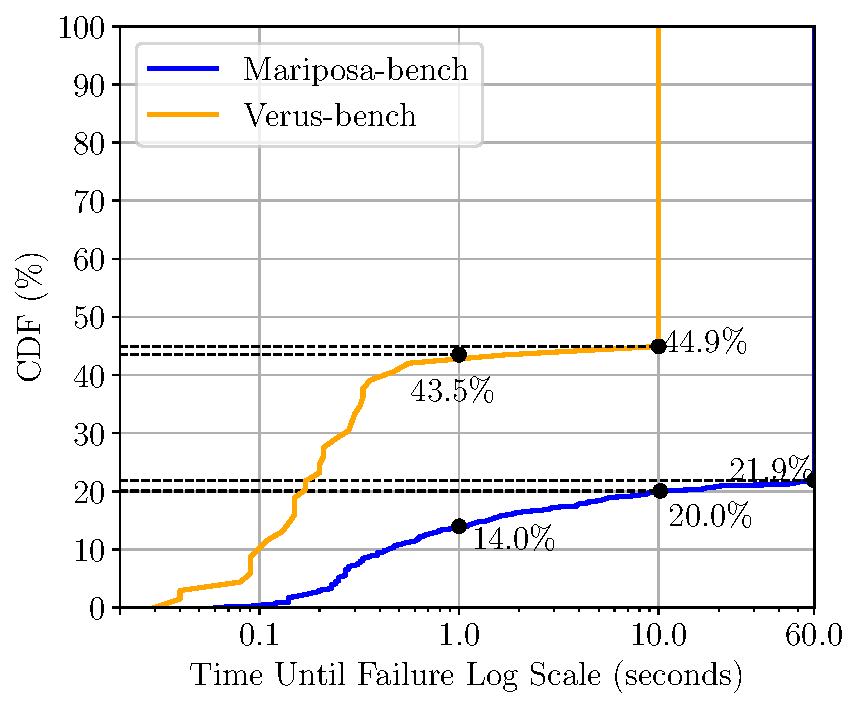
\includegraphics[width=0.8\textwidth]{fig/debugger/failure_modes.pdf}
    \caption{Distribution of failure modes in unstable mutants on a benchmark set from Mariposa~\cite{mariposa} and a benchmarks set from the Rust verifier Verus~\cite{verus-ghost}. The Verus benchmarks were run with a timeout of 10 seconds and the Mariposa benchmarks were run with a timeout of 60 seconds, corresponding to the default timeouts of the respective tools. The distribution is bimodal—most mutants either fail quickly (10 seconds for Mariposa or 1 second for Verus) or they timeout. Image is from \citet{cazamariposas}}
    \label{fig:failure_modes}
\end{figure}

This can be recognized in SMT track by noting the number of fast unknowns and
timeout failures for each solver. This would allow solvers to be scored on both
of these metrics.


\end{itemize}

\paragraph{Solutions.} There has been some work trying to fix instability.
\shake automatically prunes the solver's context by removing redundant axioms in
a pre-processing step~\cite{shake}. \caza analyzes the quantifier instantiation
graph of a query to either remove unnecessary quantifier instantiations or add missed instantiations~\cite{cazamariposas}.
Other work converts queries to a normal form to mitigate the variation in
runtimes between syntactically different, but semantically equivalent,
queries~\cite{normalize}. Dafny developers have proposed a method for instantiating universal
quantifiers for axioms at the source level~\cite{free-facts}.

All of this work makes some improvements to stability, but does not address key
underlying issues, and instability is still prevalent when we apply these fixes.
More work is required. We believe that much of this work can be done at the SMT-solver level and thus a stability track at the SMT competition could be
immensely helpful for encouraging solver developers to improve stability.

\paragraph{Drawbacks.} Many program verification tools are built with Z3 in
mind, so other solvers may perform worse initially. However, we hope that
introducing an instability track can incentivize all solvers to perform
better on verification queries and encourage verification tools to use different
solvers.

Another drawback is that measuring instability requires running many different
mutants of a query, which could be computationally expensive. However, this is
mitigated since program verification tools require much shorter timeouts
(usually 60 seconds or less) compared to many other SMT queries.

\paragraph{Conclusions.} In conclusion, we argue that instability is a critical
issue for SMT-based program verification. We believe this is a problem that
could be addressed at the solver level. We hope that an instability track at the
SMT competition could be a step in this direction.

\paragraph{Acknowledgements} We would like to thank the anonymous reviewers for their helpful feedback. We further acknowledge Dominic Winterer and the organizers of the SMT-COMP for the suggestion to present this at the SMT workshop. We thank all of the contributors to the Mariposa project and the Dafny, \fstar, and Verus developers for contributions to the benchmark suite.

This work was supported in part by the National Science
Foundation (NSF) under grant 2224279, funding from AFRL
and DARPA under Agreement FA8750-24-9-1000, and the
Future Enterprise Security initiative at Carnegie Mellon CyLab
(FutureEnterprise@CyLab).


\bibliography{refs}


\end{document}
